\documentclass[aspectratio=169,10pt]{beamer}

\usetheme{Madrid}
\usecolortheme{default}
\setbeamertemplate{navigation symbols}{}
\setbeamertemplate{footline}[frame number]
\setbeamertemplate{bibliography item}[text]

\usepackage{amsmath,amssymb,booktabs,array,graphicx,tikz}
\usetikzlibrary{arrows.meta,positioning,calc}
\pdfstringdefDisableCommands{\def\translate#1{#1}}

\definecolor{nbblue}{HTML}{0173B2}
\definecolor{nborange}{HTML}{DE8F05}
\definecolor{nbgreen}{HTML}{029E73}
\definecolor{nbred}{HTML}{B00020}
\definecolor{nbgray}{HTML}{5B6573}
\setbeamercolor{structure}{fg=nbblue}
\setbeamercolor{title}{fg=nbblue}
\setbeamercolor{frametitle}{fg=white,bg=nbblue}
\setbeamercolor{alerted text}{fg=nborange}

\newcommand{\pct}{\,\%}
\newcommand{\takeaway}[1]{%
  \vspace{0.3em}\begin{beamercolorbox}[rounded=true,sep=0.55em]{block body}
  \textbf{#1}
  \end{beamercolorbox}}

\title{EEG to caption\\26/08/2026}
\author{Philippe Forest}
\institute{IMT Atlantique}
\date{}

\begin{document}

\begin{frame}[plain]
  \centering
  \vfill
  {\color{nbblue}\bfseries\fontsize{24}{28}\selectfont
    Decoding captions from EEG\\[0.2em]26/08/2026}

  \vspace{1.2em}
  {\large Philippe Forest}

  \vspace{0.25em}
  {\small IMT Atlantique}

  \vfill
\end{frame}

\section{Setup}

\begin{frame}{Protocol}
  \begin{columns}[T,onlytextwidth]
    \column{0.47\textwidth}
      \textbf{Data}
      \begin{itemize}
        \item THINGS-EEG2, subject 01, within-subject
        \item train: 1{,}654 concepts, 16{,}540 images
        \item test: 200 concepts, one image each,
              disjoint from training
      \end{itemize}

    \column{0.49\textwidth}
      \textbf{Reference captions}
      \begin{itemize}
        \item THINGS-EEG2 does not ship any captions
        \item we write them with Qwen2-VL:
              \textit{``Describe this image in one sentence.''}
        \item five per test concept, sampled
        \item our EEG-to-caption pipeline uses BLIP-2, so we never score
              a model against its own writing
      \end{itemize}
  \end{columns}

  \vspace{0.9em}
  \centering
  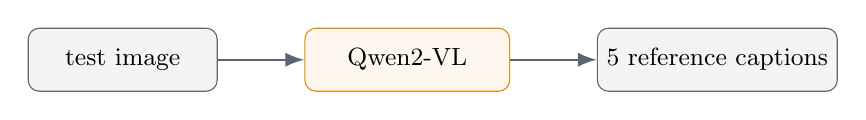
\begin{tikzpicture}[
      box/.style={draw,rounded corners,minimum height=0.8cm,align=center,font=\small},
      arr/.style={-{Latex[length=2.4mm]},thick,draw=nbgray}]
    \node[box,draw=nbgray,fill=nbgray!7,minimum width=2.4cm] (img) {test image};
    \node[box,draw=nborange,fill=nborange!7,minimum width=2.6cm,right=1.1cm of img] (qwen) {Qwen2-VL};
    \node[box,draw=nbgray,fill=nbgray!7,minimum width=3.0cm,right=1.1cm of qwen] (ref)
      {5 reference captions};
    \draw[arr] (img) -- (qwen);
    \draw[arr] (qwen) -- (ref);
  \end{tikzpicture}

  \takeaway{The ``ground truth'' is another model's description. Every group on this dataset
  invents its own, which is why published caption scores are not comparable.}
\end{frame}

\begin{frame}{One decoder, three ways in}
  \small
  BLIP-2 typically reads an image through 32 learned query tokens produced by its Q-Former;
  those 32 tokens are the only thing the language model ever sees of the image.

  \vspace{0.7em}
  \begin{center}
  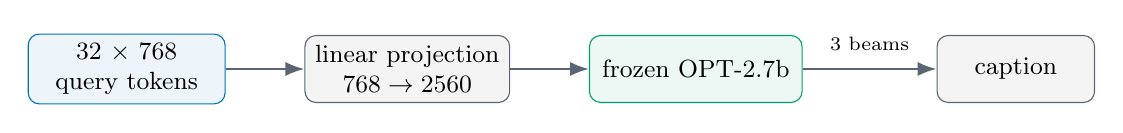
\begin{tikzpicture}[
      box/.style={draw,rounded corners,minimum height=0.85cm,align=center,font=\small},
      arr/.style={-{Latex[length=2.4mm]},thick,draw=nbgray}]
    \node[box,draw=nbblue,fill=nbblue!7,minimum width=2.5cm] (in) {32 $\times$ 768\\query tokens};
    \node[box,draw=nbgray,fill=nbgray!7,minimum width=2.6cm,right=1.0cm of in] (proj)
      {linear projection\\$768\to2560$};
    \node[box,draw=nbgreen,fill=nbgreen!7,minimum width=2.7cm,right=1.0cm of proj] (opt)
      {frozen OPT-2.7b};
    \node[box,draw=nbgray,fill=nbgray!7,minimum width=2.0cm,right=1.7cm of opt] (txt) {caption};
    \draw[arr] (in) -- (proj);
    \draw[arr] (proj) -- (opt);
    \draw[arr] (opt) -- node[above=3pt,font=\scriptsize] {3 beams} (txt);
  \end{tikzpicture}
  \end{center}

  \vspace{0.7em}
  Two routes below replace the Q-Former with a \textbf{bridge}: a single linear layer
  $\mathbb{R}^{D}\!\to\!\mathbb{R}^{32\times768}$ trained to reproduce the query tokens BLIP-2
  would have produced, with loss $\mathrm{MSE} + 0.1\cdot\mathrm{CE}$, the cross-entropy taken on
  the reference caption through the frozen language model.

  \takeaway{The captioner is never fine-tuned. We only change what we hand it.}
\end{frame}

\section{Three pipelines}

\begin{frame}{Route 1 --- Render and caption}
  \small
  Reconstruct the picture first, then describe it with an ordinary image captioner.
  The direct pipeline, no new training required.

  \vspace{0.55em}
  \centering
  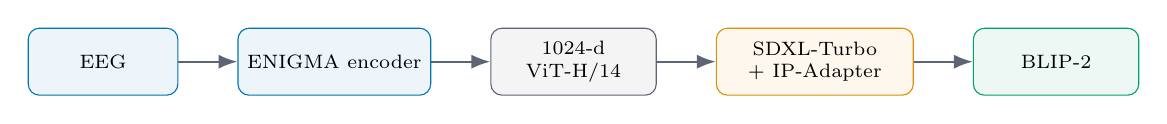
\begin{tikzpicture}[
      box/.style={draw,rounded corners,minimum height=0.85cm,align=center,font=\scriptsize},
      arr/.style={-{Latex[length=2.4mm]},thick,draw=nbgray}]
    \node[box,draw=nbblue,fill=nbblue!7,minimum width=1.9cm] (eeg) {EEG};
    \node[box,draw=nbblue,fill=nbblue!7,minimum width=2.3cm,right=0.75cm of eeg] (enc)
      {ENIGMA encoder};
    \node[box,draw=nbgray,fill=nbgray!7,minimum width=2.1cm,right=0.75cm of enc] (emb)
      {1024-d\\ViT-H/14};
    \node[box,draw=nborange,fill=nborange!7,minimum width=2.5cm,right=0.75cm of emb] (sdxl)
      {SDXL-Turbo\\+ IP-Adapter};
    \node[box,draw=nbgreen,fill=nbgreen!7,minimum width=2.1cm,right=0.75cm of sdxl] (cap)
      {BLIP-2};
    \draw[arr] (eeg) -- (enc);
    \draw[arr] (enc) -- (emb);
    \draw[arr] (emb) -- (sdxl);
    \draw[arr] (sdxl) -- (cap);
  \end{tikzpicture}

  \vspace{0.55em}
  \begin{itemize}
    \item \textbf{Encoder.} ENIGMA, the current state of the art for EEG-to-image on this dataset.
          It outputs a 1024-d CLIP-alignedembedding for each EEG sample.
    \item \textbf{Generator.} The predicted embedding enters SDXL-Turbo with IP-Adapter to replace the real image embedding.
          We use four denoising steps and no guidance. Output is $256\times256$.
    \item \textbf{Captioner.} BLIP-2 reads the generated picture and outputs a caption.
  \end{itemize}

  \takeaway{A lossy step: the reconstruction loses detail, and the captioner can only describe whatever survived.}
\end{frame}

\begin{frame}{Route 2 --- Error-matched bridge}
  \small
  Skip the picture. Learn to map the predicted embedding straight onto BLIP-2's query tokens.

  \vspace{0.55em}
  \centering
  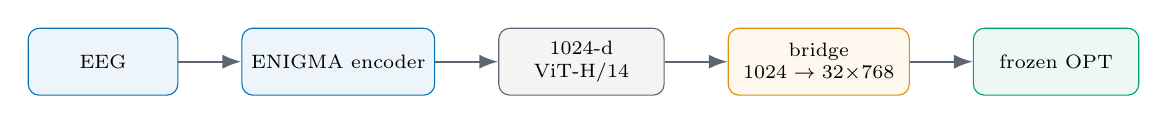
\begin{tikzpicture}[
      box/.style={draw,rounded corners,minimum height=0.85cm,align=center,font=\scriptsize},
      arr/.style={-{Latex[length=2.4mm]},thick,draw=nbgray}]
    \node[box,draw=nbblue,fill=nbblue!7,minimum width=1.9cm] (eeg) {EEG};
    \node[box,draw=nbblue,fill=nbblue!7,minimum width=2.3cm,right=0.8cm of eeg] (enc)
      {ENIGMA encoder};
    \node[box,draw=nbgray,fill=nbgray!7,minimum width=2.1cm,right=0.8cm of enc] (emb)
      {1024-d\\ViT-H/14};
    \node[box,draw=nborange,fill=nborange!7,minimum width=2.3cm,right=0.8cm of emb] (br)
      {bridge\\$1024\to32{\times}768$};
    \node[box,draw=nbgreen,fill=nbgreen!7,minimum width=2.1cm,right=0.8cm of br] (opt)
      {frozen OPT};
    \draw[arr] (eeg) -- (enc);
    \draw[arr] (enc) -- (emb);
    \draw[arr] (emb) -- (br);
    \draw[arr] (br) -- (opt);
  \end{tikzpicture}

  \vspace{0.55em}
  \begin{itemize}
    \item \textbf{The training set is the point.} The bridge is fitted on ENIGMA's \emph{own
          predictions} for the 16{,}540 training images, not on real image embeddings. It therefore
          sees the actual shape of the encoder's errors rather than clean vectors.
    \item \textbf{Correcting for optimism.} ENIGMA's cosine to the true embedding is $0.531$ on
          the training split but $0.360$ at test, because the training predictions are in-sample.
          We add isotropic noise of $\sigma=1.08$, since
          $0.531/\sqrt{1+1.08^{2}}=0.360$, so the bridge trains at the error level it will meet.
  \end{itemize}

  \takeaway{Train the decoder on the distribution it will actually be given, rather than on
  clean data it will never see again.}
\end{frame}

\begin{frame}{Route 3 --- Reconstruction-tuned bridge}
  \small
  Same bridge idea, but our own encoder and our own embedding space, and the noise is simulated
  rather than measured.

  \vspace{0.55em}
  \centering
  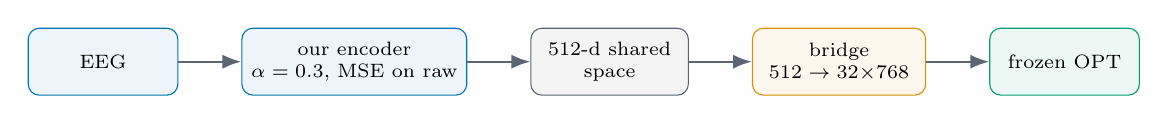
\begin{tikzpicture}[
      box/.style={draw,rounded corners,minimum height=0.85cm,align=center,font=\scriptsize},
      arr/.style={-{Latex[length=2.4mm]},thick,draw=nbgray}]
    \node[box,draw=nbblue,fill=nbblue!7,minimum width=1.9cm] (eeg) {EEG};
    \node[box,draw=nbblue,fill=nbblue!7,minimum width=2.5cm,right=0.8cm of eeg] (enc)
      {our encoder\\$\alpha=0.3$, MSE on raw};
    \node[box,draw=nbgray,fill=nbgray!7,minimum width=2.0cm,right=0.8cm of enc] (emb)
      {512-d shared\\space};
    \node[box,draw=nborange,fill=nborange!7,minimum width=2.2cm,right=0.8cm of emb] (br)
      {bridge\\$512\to32{\times}768$};
    \node[box,draw=nbgreen,fill=nbgreen!7,minimum width=1.9cm,right=0.8cm of br] (opt)
      {frozen OPT};
    \draw[arr] (eeg) -- (enc);
    \draw[arr] (enc) -- (emb);
    \draw[arr] (emb) -- (br);
    \draw[arr] (br) -- (opt);
  \end{tikzpicture}

  \vspace{0.55em}
  \begin{itemize}
    \item \textbf{Encoder.} Ours, aligned to InternViT-6B layer 28 rather than a final CLIP layer.
          The loss is $0.3\cdot\mathrm{InfoNCE}+0.7\cdot\mathrm{MSE}$ on unnormalised features:
          far more weight on reconstruction than we normally use for retrieval. Best of twelve
          variants screened.
    \item \textbf{Bridge training.} Fitted on \emph{real} images pushed through the encoder's own
          image projector into the 512-d space, then corrupted with $\sigma=2.12$, chosen from the
          measured EEG-image cosine of $0.426$.
  \end{itemize}

  \takeaway{Routes 2 and 3 answer the same train-test mismatch two ways: one trains on the real
  errors, the other on a Gaussian imitation calibrated to the same cosine.}
\end{frame}

\section{Evaluation}

\begin{frame}{Metrics, and the control they are reported against}
  \small
  Two of these never look at a reference caption, which matters because our references are
  themselves machine-written.

  \vspace{0.45em}
  \begin{itemize}
    \item \textbf{Identification.} Encode the caption with CLIP's text encoder and retrieve the
          true image among the 200 test images. Chance is $0.5\pct$. Hedging cannot help:
          a vague sentence retrieves nothing in particular.
    \item \textbf{WUP.} Best Wu--Palmer similarity in WordNet between a noun in the caption and
          the target concept, so a near miss scores above an unrelated word.
    \item \textbf{CIDEr.} tf-idf weighted $n$-gram agreement with the five references, which
          rewards distinctive matches rather than common words.
    \item \textbf{BERTScore.} Contextual-embedding F1, best over the five references. Catches
          paraphrase that $n$-gram counting misses.
  \end{itemize}

  \vspace{0.35em}
  Each is paired with a \textbf{permutation null}: the arm's own captions dealt to the wrong
  concepts, over 1000 permutations. This holds length, vocabulary and style exactly fixed and
  destroys only the pairing.

  \takeaway{Report the margin over the null, never the raw score. A cautious captioner can raise
  its raw number without decoding anything.}
\end{frame}

\section{Results}

\begin{frame}{Results}
  \vspace{4pt}
  \begin{center}
  \small
  \begin{tabular}{@{}lrrrr@{}}
    \toprule
    Route & Identification & WUP & CIDEr & BERTScore \\
    \midrule
    Render and caption          & 9.50 & 65.08 & 3.76 & 88.04 \\
    Error-matched bridge        & \textbf{10.00} & \textbf{67.57} & 9.10 & \textbf{89.26} \\
    Reconstruction-tuned bridge & 7.50 & 64.87 & \textbf{9.49} & 89.17 \\
    \midrule
    \textit{permutation null}   & \textit{$\approx$0.50} & \textit{57--61} & \textit{1.2--3.1} & \textit{$\approx$87.9} \\
    \midrule
    Image ceiling (no EEG)      & 92.50 & 82.41 & 46.31 & 91.83 \\
    \bottomrule
  \end{tabular}
  \end{center}

  \vspace{0.5em}
  \small The ceiling is the same bridge fed a real image embedding instead of an EEG one.
  It separates what the decoder cannot do from what the EEG cannot supply.

  \takeaway{Every route beats its null on every metric, so all three carry real stimulus
  information. None of them approaches the ceiling.}
\end{frame}

\begin{frame}{The metrics disagree, and that is the finding}
  \small
  \begin{columns}[T,onlytextwidth]
    \column{0.48\textwidth}
      \textbf{Reference-based metrics}
      \begin{itemize}
        \item bridges beat rendering by a wide margin
        \item CIDEr $9.1$ and $9.5$ against $3.8$
        \item the gap is large and consistent
      \end{itemize}

    \column{0.48\textwidth}
      \textbf{Reference-free metrics}
      \begin{itemize}
        \item identification $10.0$, $7.5$, $9.5$
        \item no route separates from another
        \item rendering is the best of the three on
              concept naming
      \end{itemize}
  \end{columns}

  \vspace{0.8em}
  The bridges were trained with a cross-entropy term on the reference captions, so they learn the
  reference vocabulary and phrasing. That lifts every overlap-based score without necessarily
  adding information about the stimulus. Identification is immune, and under identification the
  three routes are indistinguishable at $n=200$.

  \takeaway{Captions that read better are not captions that identify better. With 200 test
  concepts we cannot resolve differences of a few points, so the next step is more subjects,
  not more decoder variants.}
\end{frame}

\end{document}
